\section{背景}
\subsection{投機実行}
\label{sec:spec_exec}

現代のCPUは、命令の実行を命令フェッチ、デコード、実行などの複数ステージに分割するパイプライン方式を採用しており、これにより前の命令が全ての処理を終えるのを待たずに次の命令の処理を開始することが可能となる。このように、複数の命令を並行して処理することで、CPUのスループットを大幅に向上させる。
しかし、次に実行すべき命令が先行する命令の実行結果に依存している場合、CPUは次に実行する命令を判断できず、処理を一時的に停止せざるを得ない(Stall)。このような状況は制御ハザードと呼ばれ、CPUのパフォーマンスに大きな影響を与える。この問題を回避するため、CPUは先行する命令の結果を待たずに、将来的に必要となる可能性の高い命令を投機的に実行する。これは投機実行と呼ばれる最適化手法であり、ほぼ全ての最新CPUに実装されている。\par

分岐予測は、この投機実行を応用した最適化手法の一つである。分岐命令に遭遇した際、CPUは過去の実行結果に基づいて分岐先を予測し、後続の命令を投機的に実行する。分岐予測による投機実行を図\ref{fig:Speculative_Execution}に示す。分岐予測が成功すれば、CPUはStallを回避して効率的に命令を処理できる。一方、分岐予測が失敗した場合、投機実行された命令の結果は全て破棄され、正しい分岐方向から実行を再開する必要がある。この予測にはCPUの分岐予測器が使用され、分岐命令ごとに過去の分岐結果を記録し、それに基づいて予測を行う。\par

投機的に実行された命令とその結果は、CPU内部のReorder Buffer (ROB)という機構で管理される。ROBは、投機実行された命令が依存する他の命令の完了を待ちながら、命令の実行順序を維持する役割を持つ。そのため、投機実行可能な命令数はROBのサイズによって制限されており、通常200命令程度のマイクロオペレーション ($\mu$OP)が上限とされる。分岐先が確定し、予測が正しいと判明した場合、投機的実行の結果はレジスタやメモリなどのアーキテクチャ状態に反映される。一方、予測が誤っていた場合、ROB内の投機実行の結果は全て破棄され、誤った予測が行われた時点のアーキテクチャ状態までロールバックされる。

\begin{figure}[tb]
  \centering
  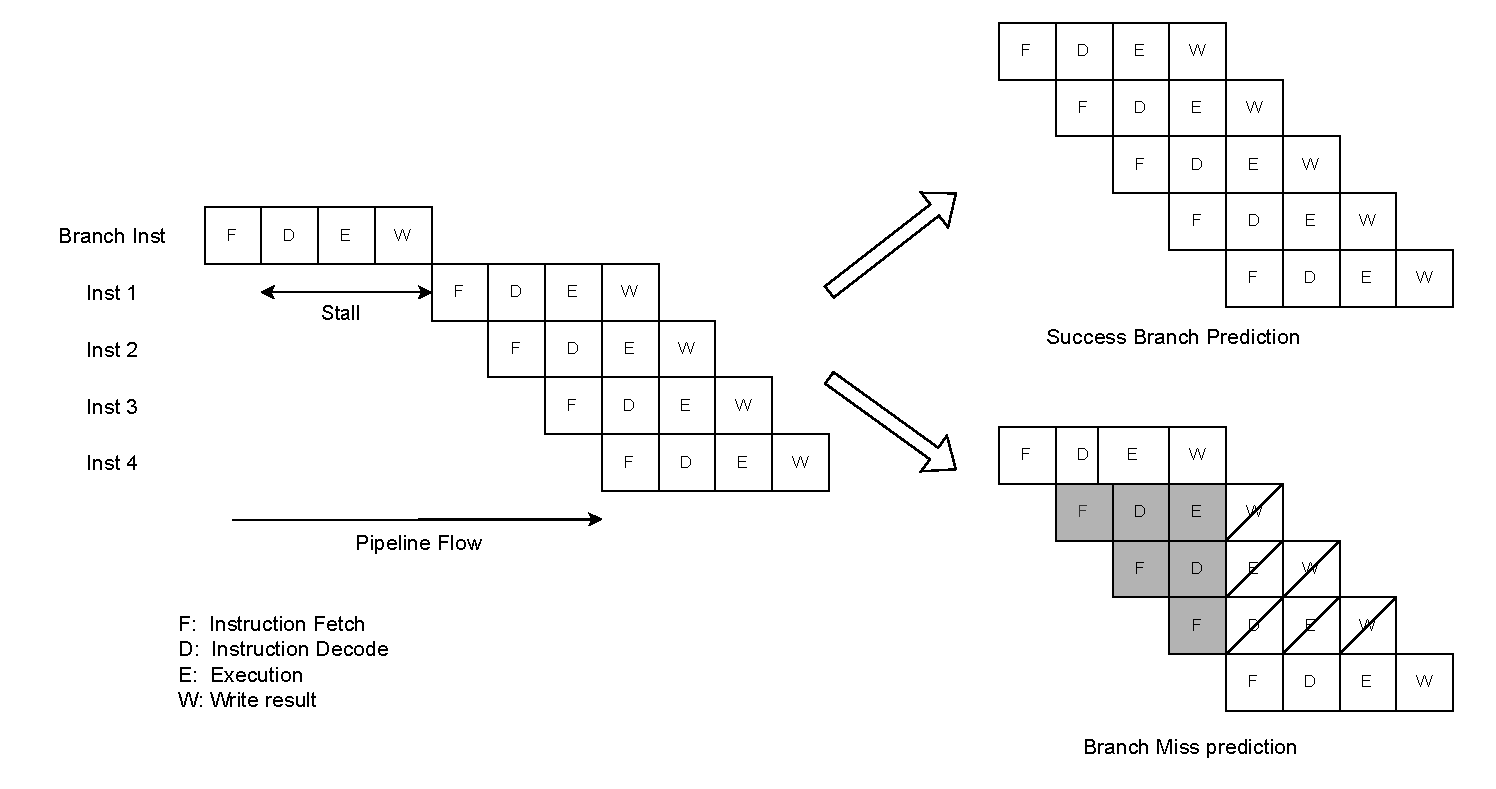
\includegraphics[width=\linewidth]{img/Speculative_Execution.drawio.pdf}
  \caption{分岐予測による投機実行}\label{fig:Speculative_Execution}
\end{figure}


\subsection{Side Channel Attack}
コンピュータのシステムにおいて、channelとは情報を送信する可能性のある媒体のことを言う。channelには大きく分けてlegitimate channelと incidental channelの2種類が存在する\cite{intel-channel}。legitimate channelはシステムの設計者が情報送信用に意図的に設計したチャネルであり、イーサネット、共有メモリ、IPCソケットなどがある。逆にincidental channelは、意図せずに設計されたチャネルであり、リソースの競合、キャッシュの状態、電力消費の変化などがある。更に、セキュリティ脅威モデルのコンテキストにおいてincidental channelはcovert channelとside channelの2種類に分類される。covert channelは悪意のある送信者と受信者が意図的に情報の伝達を行うために利用されるchannelである。一方でside channelは、送信者は受信者に情報を伝達することを意図しておらず、情報が悪意のある受信者に伝達(つまり漏洩)される際に利用されるchannelであり、このようなchannelを悪用する攻撃手法をside channel attackという。\par 

side channel は 情報を伝達する方法に基づいて、Timing-based channel、Access-based channel、またはTrace-based channel に分類される\cite{szefer2019survey}。Timing-based channel は、様々な操作のタイミングを利用することで被害者の情報を推測する。例えば、攻撃者は様々な入力を暗号化または復号化し、その時の実行時間の差分を計測し分析することで、暗号鍵に関する情報を明らかにする\cite{song2001timing}。Access-based channelは メモリやキャッシュなどの共有リソースに直接アクセスすることで、被害者のプロセスの情報を推測する。例えば、キャッシュがプロセス間で共有されていることを利用し、特定のキャッシュラインへのアクセス時間を計測することで、被害者プロセスの動作を推測する\cite{liu2015last}。Trace-based channel は デバイスの消費電力や電磁放射などのプログラム実行時の詳細な情報を計測することで情報の漏洩を試みる。例えば、攻撃者は暗号化中のデバイスの消費電力を計測し分析することで、暗号化に関する情報を収集する\cite{aciiccmez2006trace}。\par

以降の節では、近年のCPUのキャッシュの基本的な構造と、それをside channelとして利用する代表的な攻撃手法であるPrime+Probe\cite{tromer2010efficient}とFlush+Reload\cite{yarom2014flush+}について説明する。これらの攻撃は本研究の対象である、Spectre攻撃の中でも頻繁に利用される攻撃手法であるため、以降の節で詳しく説明する。

\subsubsection{キャッシュ構造}

\begin{figure}[tb]
  \centering
  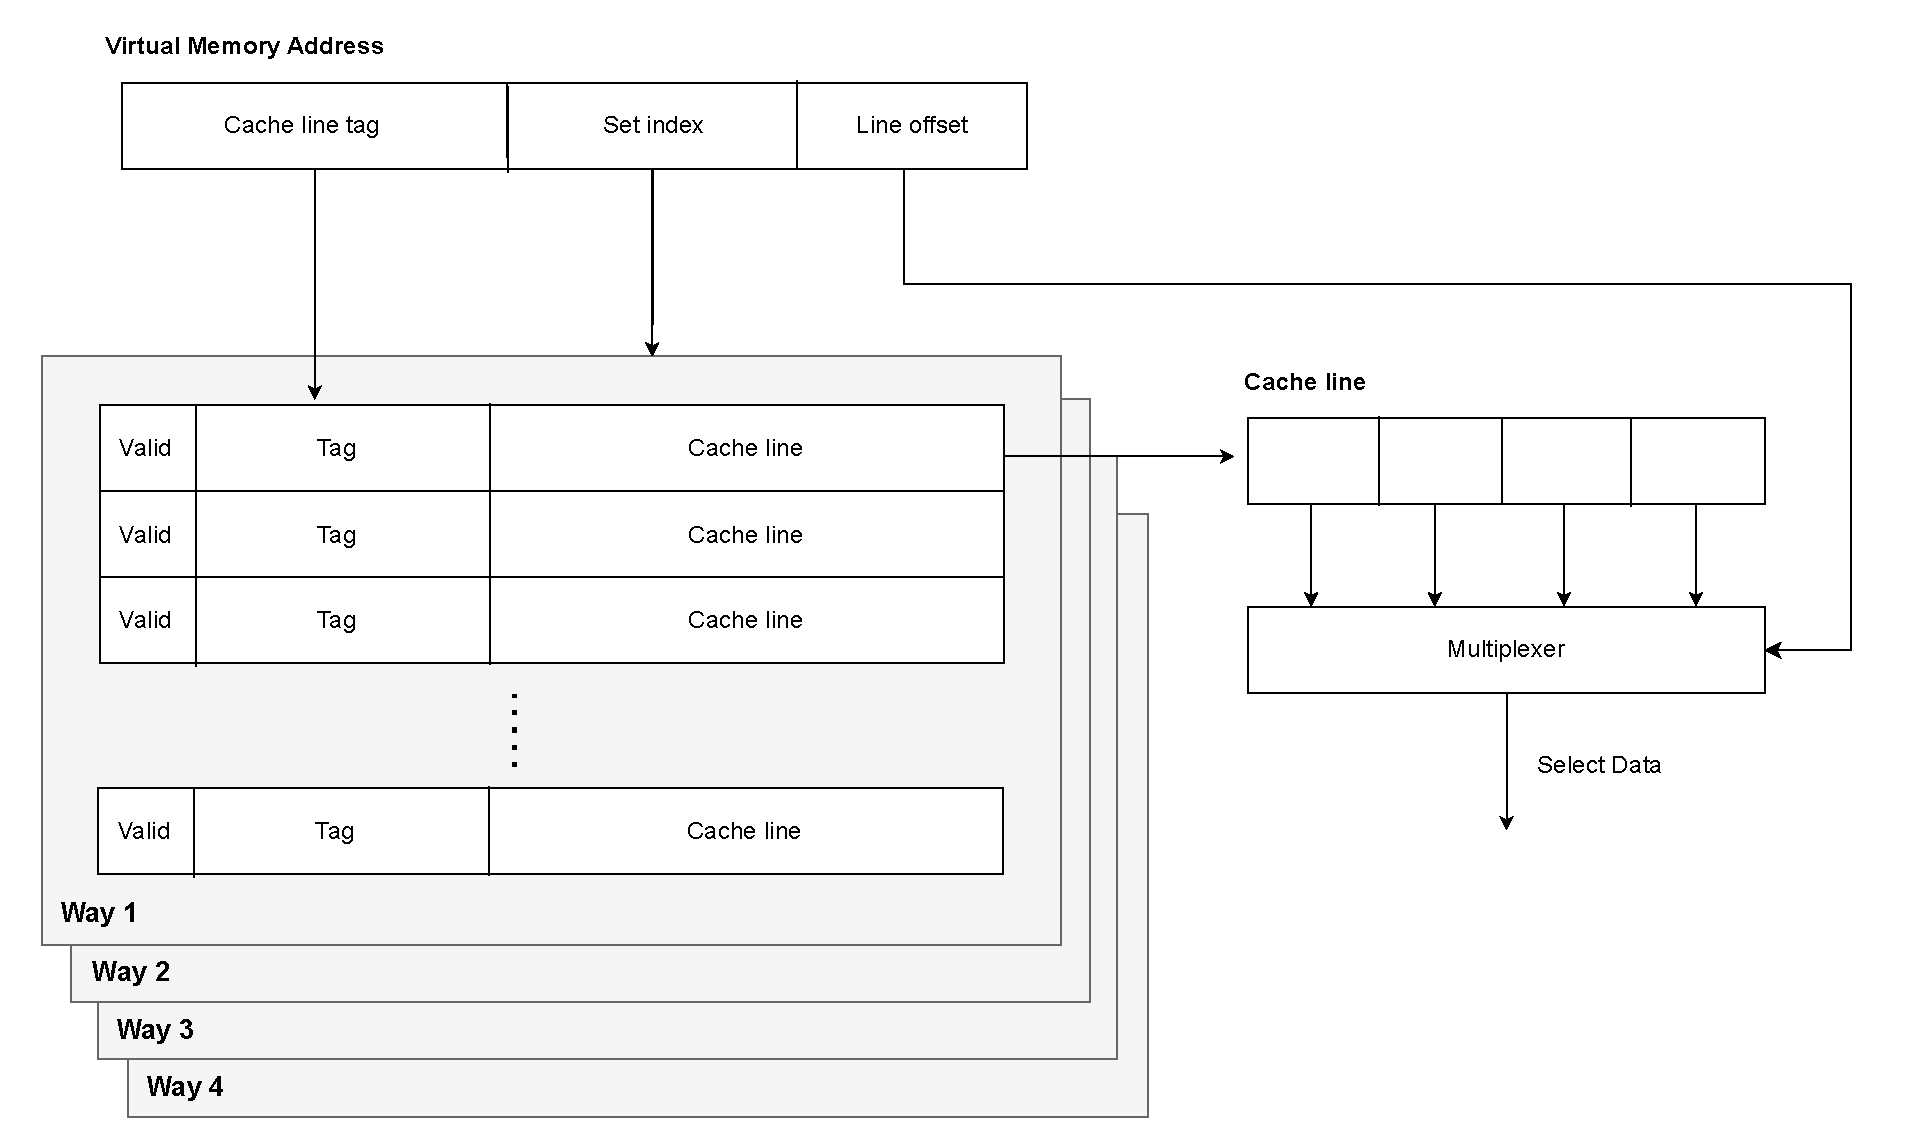
\includegraphics[width=\linewidth]{img/cache.drawio.pdf}
  \caption{仮想アドレスによるキャッシュの参照}\label{fig:cache-overview}
\end{figure}

キャッシュをside channelとして利用する攻撃手法を紹介する前に、近年のCPUにおけるキャッシュ構造について説明する。近年のCPUは、CPUとメモリの性能差に効率的に対処するため、複数の性能が異なるキャッシュメモリを階層的に配置する設計が採用されている。このキャッシュ階層は、CPUに近い順にL1キャッシュ、L2キャッシュと続き、最も遠いキャッシュはLLC(Last Level Cache)と呼ばれる。これらのキャッシュはCPUに近いほど高速だが容量が小さく、遠いほど容量は大きいが低速であるという特徴を持つ。一般的にL1キャッシュとL2キャッシュは各コア専用で、LLCは複数のコアで共有されているため、LLCはside channel attackの攻撃対象として適している。\par

キャッシュは複数のキャッシュセットで構成され、各セットには複数のキャッシュラインが含まれている。このようなキャッシュ構造をセットアソシエイティブ型と呼び、各キャッシュセット内のキャッシュライン数を連想度(way)という。連想度が増加すると、キャッシュの競合性ミスが減少するが、比較器やキャッシュの設計コストが増加するため、バランスの取れた設計が求められる。\par

仮想メモリアドレスは、以下の3つの要素で構成される。

\begin{itemize}
  \item Cache set index: データがどのキャッシュセットにマップされるかを決定する。
  \item Cache line tag: キャッシュセット内でデータを識別するタグ。
  \item Cache line offset: キャッシュライン内でどのデータワードが対象であるかを識別するタグ。
\end{itemize}

キャッシュは仮想アドレスの一部をインデックスとして使用し、各メモリアドレスを特定のキャッシュセットにマップする。そして、セット内の任意のキャッシュラインにデータを格納する。この際、マップ先のキャッシュセットがすでに埋まっている場合は、キャッシュ置換ポリシーに基づいて、どのキャッシュラインを削除するかが決定される。一般的に採用される手法は、Least Recently Used (LRU)やLeast Frequently Used (LFU)といったポリシーである。仮想メモリアドレスによる4wayセットアソシエイティブ型キャッシュへの参照の概要を図\ref{fig:cache-overview}に示す。

\subsubsection{Prime+Probe}

\begin{figure}[tb]
  \centering
  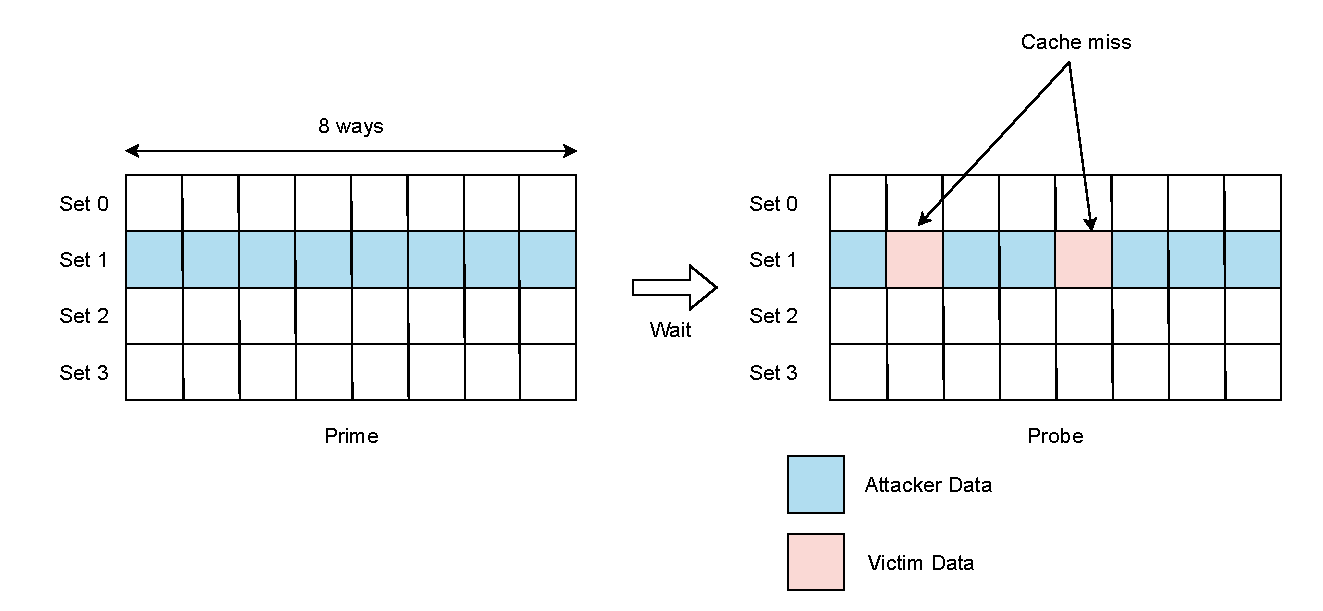
\includegraphics[width=\linewidth]{img/prime+probe.drawio.pdf}
  \caption{Prime+Probeの概要}\label{fig:prime-probe}
\end{figure}

Prime+Probe\cite{tromer2010efficient}はキャッシュをside channelとして利用し、キャッシュ内の被害者のデータアクセスパターンから秘密情報を抽出する攻撃手法である。攻撃の概要について図\ref{fig:prime-probe}に示す。まず、攻撃者は、攻撃者プロセスにおけるコードブロックと被害者プロセスにおける機密性の高いコードブロックの両方がマップされるキャッシュセットを見つける。先述の通り、一部のキャッシュ階層は複数コア間で共有されているため、攻撃者と被害者プロセスが同一コアにスケジュールされていなくても攻撃することは可能である\cite{liu2015last}。そして、攻撃者プロセスを一定時間実行することで、被害者と競合するキャッシュセットを自身のデータで埋める(Primeフェーズ)。その後、攻撃者は一定時間待機し、被害者プロセスが実行されるのを待つ。これにより、競合したキャッシュセットの一部は被害者のデータによって上書きされている可能性がある。その後、攻撃者はPrimeフェーズで埋めたデータに再度アクセスし、アクセス時間を計測する(Probeフェーズ)。アクセス時間を計測することで、攻撃者のデータがキャッシュ上に存在するかがわかるため、待機時間の間にどのキャッシュラインを被害者プロセスがアクセスしたかがわかる。つまり、攻撃者は特定のキャッシュセットにおける被害者プロセスのメモリアクセスパターンを把握することが可能となる。\par
Prime+Probeは後述するFlush+Reloadと比較して、フラッシュ命令や共有メモリを必要としないためより汎用的である。しかし、対象とするキャッシュがLLCのように大容量の場合、キャッシュセットを攻撃者のデータで埋めるまでに時間がかかるという欠点がある。

\subsubsection{Flush+Reload}
Flush+Reload\cite{yarom2014flush+}はPrime+Probeと同様に、データキャッシュを利用するside channel attackであるが、前提条件として被害者と攻撃者のプロセス間で特定のメモリ領域を共有している必要がある。プロセス間でメモリを共有するシナリオとして、プロセス間通信に利用される場合や、メモリフットプリントの削減のために、ハイパーバイザが仮想マシン間で同一内容のメモリページを共有する際に利用する場合がある\cite{yarom2014flush+}。\par
まず、攻撃者は共有されたメモリ領域の中から観測対象とするアドレスを選択し、clflush命令などを使用して、選択したアドレスのキャッシュラインをキャッシュ階層全体から排除する(Flushフェーズ)。その後、攻撃者は一定時間待機し、被害者プロセスが観測対象のアドレスにアクセスするのを待つ。その後、攻撃者は観測対象のアドレスに再度アクセスし、アクセス時間を計測する(Reloadフェーズ)。待機中に被害者プロセスが観測対象のアドレスにアクセスした場合、そのキャッシュラインはキャッシュで利用可能になり、アクセス時間は短くなる。一方、被害者プロセスが観測対象のアドレスにアクセスしていない場合、キャッシュラインをメモリから取得する必要があるため、アクセス時間は長くなる。このようにして、攻撃者は待機中に被害者プロセスが観測対象のアドレスにアクセスしたかどうかを把握することが可能となる。\par
Flush+Reloadは攻撃のために前提条件が必要だが、Prime+Probeと比較して特定のアドレスのキャッシュラインをフラッシュすれば良いだけので、攻撃にかかる時間が短いという利点がある。

\subsection{Transient Execution Attack}

transient execution attackは、CPUの投機的実行によって一時的に実行される命令の結果がマイクロアーキテクチャに痕跡を残すことを利用した攻撃手法である。通常、CPUは誤った投機的実行が行われた場合、パイプラインをフラッシュし、アーキテクチャの状態を投機実行の前の状態までロールバックさせる。しかし、キャッシュなどの一部のマイクロアーキテクチャの状態は、パフォーマンスの観点からそのまま維持される。この特性を利用し、攻撃者は意図的に悪意のある投機的実行を誘発し、マイクロアーキテクチャの状態を介して秘密情報を復元することが可能となる。\par

transient execution attackは、2018年にSpectre攻撃\cite{8835233}とMeltdown攻撃\cite{217478}が明らかにされて以来、様々なCPUを標的とした新しい攻撃手法が次々と発見されてきた。これらの攻撃は大きくSpectre型\cite{8835233,220586,10.1145/3243734.3243761,horn2018speculative}とMeltdown型\cite{217478,van2018foreshadow,stecklina2018lazyfp,van2019ridl,van2020lvi}に分類される\cite{canella2019systematic}。Spectre型は、データフローや制御フローにおける予測ミスによって発生する一時的な命令を悪用する。一方で、Meltdown 型攻撃は、例外を引き起こす命令に続く一時的な命令を利用する。\par

transient execution attackは大きく分けて3つのフェーズで構成される。
まず攻撃者は分岐予測器やデータキャッシュの状態を調整し、マイクロアーキテクチャを特定の状態にする。次に、投機実行を引き起こすトリガー命令を実行する。これは、例外や分岐予測ミスなどを発生させることで、後続の命令が最終的に潰されるような命令である。CPUはトリガー命令が完了する前に後続の命令を一時的に実行する。この命令はマイクロアーキテクチャのside channelの送信側として機能し、秘密情報をキャッシュの状態に反映させたりする。トリガー命令の処理が終了すると、CPUは例外や分岐予測ミスを検知し、パイプラインをフラッシュし、アーキテクチャの状態をロールバックする。最後に攻撃者は、side channelの受信側で、メモリアクセス時間の計測を行うことで、マイクロアーキテクチャの状態から秘密情報を復元する。\par

\subsection{Spectre攻撃と対策}

\begin{figure}
  \begin{minted}[linenos,escapeinside=@@,label=BCB,autogobble]{c}
i = input();
if (i < array1_size) { // VB: Victim branch
  secret = array1[i]; // RS: Read Secret 
  tmp &= array2[secret]; // LS: Leak Secret  
}
\end{minted}
  \caption{Spectre-PHT 脆弱性を含むコード片}
  \label{BCB}
\end{figure}

Spectre攻撃\cite{8835233,Spectre-v4,220586,10.1145/3243734.3243761}はCPUの脆弱な投機実行を悪用することで、被害者プロセスの秘密情報を漏洩させる攻撃手法である。投機実行はCPUのパフォーマンス向上に大きく寄与しており、ほぼ全ての最新のCPUに実装されている最適化手法である。そのため、Spectre攻撃は、特定のベンターに限らず、ほぼ全てのCPUが攻撃対象となる可能性がある。2018年にCPUのSpectre脆弱性が発見されて以降、多くの対処法が研究されているが、未だにSpectre脆弱性を完全かつ効率的に排除する手法は確立されていない。本章では、本研究の対象でありSpectre脆弱性の一種であるSpectre-PHT\cite{8835233}と、その脆弱性に対する代表的な防御手法について紹介する。

\subsubsection{Spectre-PHT}
Spectre-PHT(Spectre v1)\cite{8835233}はSpectre攻撃の一種であり、条件分岐命令の誤った予測によって引き起こされる投機実行による境界外へのメモリアクセスを利用する攻撃手法である。投機実行により条件分岐命令をバイパスするため、Bounds-Check-Bypass (BCB)攻撃とも呼ばれる。\par

図\ref{BCB}に示すSpectre-PHT脆弱性を含むコード辺を用いて、具体的な攻撃手順を説明する。前提として、変数\var{i}の値は外部から入力として与えられ、攻撃者が操作可能であるとする。\par

\begin{figure}[tb]
  \centering
  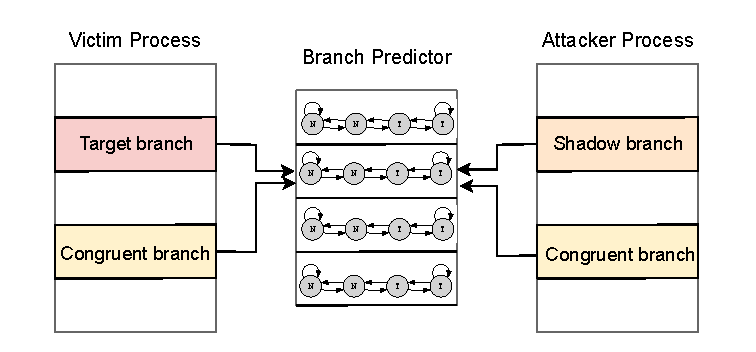
\includegraphics[width=\linewidth]{img/branch_predicator.drawio.pdf}
  \caption{分岐予測器のトレーニング}
  \label{fig:branch_predicator}
\end{figure}


攻撃者はまず、2行目の\var{if}文(Victim branch, VB)の条件がTrueと予測されるように分岐予測器をトレーニングする必要がある。近年のCPUにおける分岐予測器は、分岐命令の仮想アドレスをインデックスとして利用する\cite{fog2016microarchitecture,8835233}。この特性を利用し、攻撃者は、Victim branchと同一の仮想アドレスを持つ分岐命令(Shadow branch)を用いて、自身のプロセス内で分岐予測器をトレーニングできる。また、仮想アドレスの一部のみが分岐予測器のインデックスとして使用される場合には、Victim branchと仮想アドレスの一部が一致する分岐命令(Congruent branch)を使用してトレーニングを行うことも可能である。これにより、攻撃者は図\ref{fig:branch_predicator}に示すように、複数の経路を通じて分岐予測器をトレーニングできる\cite{canella2019systematic}。図\ref{BCB}のコード辺では、2行目の条件分岐がTrueになるような入力を繰り返し与え、分岐予測器をTrue側にトレーニングする。\par

次に、攻撃者は変数\var{i}に\var{array1\_size}以上の値を与える。この場合、通常の実行では2行目の境界チェックによって、3行目と4行目の処理は実行されずにプログラムは終了する。しかし、先述のトレーニングの結果、分岐予測器は分岐条件がTrueになると誤って予測するため、3,4行目が投機実行される。この投機実行により、3行目では攻撃者が操作可能な変数\var{i}を使用して境界外アクセスが発生する(Read Secret, RS)。読み取られた値は、4行目で\var{array2}へのアクセスのインデックスとして使用され、キャッシュの状態に変更が加えられる(Leak Secret, LS)。その後、CPUは分岐条件の評価結果から分岐予測が誤っていたことを知り、投機実行中のメモリアクセス結果を破棄するが、キャッシュの状態はパフォーマンスの観点からロールバックされない。\par

最後に、攻撃者は先述のPrime+ProbeやFlush+Reloadといったside channel attackを用いて、投機実行中のメモリアクセスで使用されたキャッシュラインを把握する。4行目で読み取られたメモリアドレスは秘密情報に依存しており、使用されるキャッシュラインの位置は仮想アドレスによって決定するため、どのキャッシュラインが使用されていたかを把握することで、秘密情報を復元することが可能になる。\par
以上のことから、Spectre-PHT脆弱性は、(i) 攻撃者が制御可能な分岐命令(VB)、(ii) 秘密情報を読み取る命令(RS)、(iii) 読み取った秘密情報をキャッシュ状態に反映させる命令(LS)の3つの命令から構成される。ただし、実際の攻撃では、VBに該当する命令の分岐予測から開始した投機実行が終了する前に、LS及びRSに該当する命令の実行を完了する必要がある。これは、キャッシュ状態に秘密情報を反映させる前に投機実行が終了してしまうと、実行状態がロールバックされ、攻撃が成立しないためである。投機実行可能な命令数はCPUのROBのサイズに制限されており(詳しくは\ref{sec:spec_exec}を参照)、投機実行可能な命令数の上限をSpeculative execution window(投機ウィンドウ)という。このように、Spectre-PHT脆弱性を含んだコード辺はSpectre Gadgetと呼ばれる。以降ではSpectre-PHTを単にSpectreと表記する。


\subsubsection{直列化命令}

\begin{figure}
  \begin{minted}[linenos,escapeinside=@@,label=BCB,autogobble]{c}
#include <x86intrin.h>
i = input();
if (i < array1_size) {
  _mm_lfence();   // Add lfence
  secret = array1[i];  
  tmp &= array2[secret];  
}
\end{minted}
  \caption{Spectre Gadgetに対し、lfence命令による防御策を適用した例}
  \label{lfence}
\end{figure}

Spectre攻撃には投機実行が必要である。そのため、命令がその命令に至る制御フローが確定した場合にのみ実行されるようにすることで、Spectre攻撃を防御することが可能である。このアプローチとして、元のプログラムに直列化命令を挿入して修正する方法が提案されている\cite{8835233}。例えばx86アーキテクチャの場合、lfence命令を使用することが可能である。lfence命令は、全ての先行するメモリロード命令が完了するまで、後続のメモリロード命令を投機実行させないようにする制御命令である。プログラム中の全ての条件分岐命令の分岐先にlfence命令を挿入することで、それ以降のメモリロード命令の投機実行を抑制し、Spectre攻撃を防御できる。\par

図\ref{BCB}のコード片に対して lfence命令を挿入してSpectre攻撃に対して堅牢化したコード辺を図\ref{lfence}に示す。4行目にlfence命令が挿入されることで、3行目の分岐条件の評価が終了し分岐先が確定してから、後続の配列へのアクセスが行われるようになる。\par 
しかし、CPUの分岐予測を完全に無効化することで、大幅にパフォーマンスが低下することが知られている。既存研究\cite{wang2018oo7}では、元のプログラムの全ての条件分岐命令に対してlfence命令を挿入した場合、プログラムの実行時間が最大3.25倍程度に増加することが報告されている。

\subsubsection{Speculative Load Hardening}

\begin{figure}
  \begin{minted}[linenos,escapeinside=@@,label=BCB,autogobble]{c}
void leak(int data);
void example(int* pointer1, int* pointer2) {
  if (condition) {
    // ... lots of code ...
    leak(*pointer1);
  } else {
    // ... more code ...
    leak(*pointer2);
  }
}
\end{minted}
  \caption{SLH適用前のSpectre Gadget}
  \label{SLH_before}
\end{figure}

\begin{figure}
  \begin{minted}[linenos,escapeinside=@@,label=BCB,autogobble]{c}
uintptr_t all_ones_mask = std::numerical_limits<uintptr_t>::max();
uintptr_t all_zeros_mask = 0;
void leak(int data);
void example(int* pointer1, int* pointer2) {
  uintptr_t predicate_state = all_ones_mask;
  if (condition) {
    predicate_state = !condition ? all_zeros_mask : predicate_state;
    // ... lots of code ...
    pointer1 &= predicate_state;
    leak(*pointer1);
  } else {
    predicate_state = condition ? all_zeros_mask : predicate_state;
    // ... more code ...
    int value2 = *pointer2 & predicate_state;
    leak(value2);
  }
}
\end{minted}
  \caption{SLH適用後のコード辺}
  \label{SLH_after}
\end{figure}

Spectre攻撃に対する実行時オーバーヘッドが少ない防御策として、Carruthによって提案されたSpeculative Load Hardening(SLH)\cite{LLVM-SLH}がある。SLHはコンパイラベースの防御手法であり、分岐命令を使用せずに、メモリアクセス命令が有効な制御フローパス上で実行されているかを確認するコードを計装する。以降では、先行研究\cite{LLVM-SLH}に示されているコード例を元に、SLHの概要を説明する。\par

図\ref{SLH_before}と図\ref{SLH_after}は、それぞれSLH適用前と後のコード辺である。ここで、関数\var{leak}は投機実行された場合に引数のデータを攻撃者に漏洩させると仮定する。変数\var{predicate\_state}は、現在の実行が分岐予測ミスによる分岐先であるかを表しており、7行目と12行目において、条件\var{condition}が満たされない場合は\var{all\_zeros\_mask}(全てのビットが0)、満たしている場合は\var{all\_ones\_mask}(全てのビットが1)が代入される。重要な点として、7行目の三項演算子は分岐命令が使用されない形で機械語に変換される必要がある。これにより、7行目の条件\var{condition}が投機実行によってバイパスされないことを保証する。x86アーキテクチャでは、cmov命令を用いることで実現可能である\cite{LLVM-SLH}。\par
分岐予測が正しい場合は、\var{predicate\_state}には\var{all\_ones\_mask}が格納される。そのため、9行目及び13行目でビット論理積が取られても、\var{pointer1}及び\var{pointer2}の値はそのまま保持される。一方、分岐予測が誤っている場合、\var{predicate\_state}には\var{all\_zeros\_mask}が格納されている。これにより、ビット論理積を取ることで、\var{pointer1}と\var{pointer2}の値は0となる。その結果、関数\var{leak}が実行されても攻撃者が意図したデータは漏洩しない。\par

lfence命令を用いた防御策では、lfence命令以降に続く全てのメモリロード命令の投機実行が抑制される。このため、Spectre攻撃に関与しない安全なメモリロード命令であっても、投機実行が制限されてしまう。また、分岐予測が正しく行われた場合でも、lfence命令以降の投機実行が抑制されるため、パフォーマンスが大幅に低下する。一方、SLHは、投機実行による漏洩のリスクがある危険なメモリロード命令に対してのみ投機実行を抑制する。そのため、投機実行可能なメモリロード命令を増やすことができ、lfence命令と比較して小さい実行時オーバーヘッドでSpectre攻撃を防御することができる。しかし、それでも全てのメモリロード命令をSLHで強化する場合、大規模なアプリケーションでは実行時オーバーヘッドが36\%程度になることが報告されている\cite{LLVM-SLH}。

\subsection{Spectre Gadgetの検出}
Spectre攻撃に対してプログラムを堅牢化するために、lfence命令やSLHを全ての条件分岐命令やメモリロード命令に適用する場合、大きな実行時オーバーヘッドが発生する。そこで、プログラム内の潜在的なSpectre Gadgetを検出し、これらのGagetのみに防御策を適用して、実行時オーバーヘッドを軽減する方法が提案されている。\par

Spectre Gadgetを検出するためのプログラム解析手法は大きく分けて、静的解析\cite{Spectre-Scanner,wang2018oo7,guarnieri2020spectector,wang2020kleespectre}による手法と、動的解析\cite{oleksenko2020specfuzz,qi2021spectaint,johannesmeyer2022kasper}による手法の2種類に分類される。投機実行はハードウェアによる機能であるため、これらの解析手法の大半がソフトウェアレベルで投機実行をシミュレートすることでSpectre Gadgetを検出している。以降では、それぞれの手法がどのように投機実行をシミュレートし、Spectre Gadgetを検出しているかを説明する。その代表例として、静的解析による検出手法としてKLEESpectre\cite{wang2020kleespectre}を、動的解析による検出手法としてSpecFuzz\cite{oleksenko2020specfuzz}を紹介する。これらの既存手法は本研究における実装の基盤にもなっているため詳しく説明する。

\subsubsection{KLEESpectre}

\begin{figure}
  \begin{minted}[linenos,escapeinside=@@,label=BCB,autogobble]{c}
    uint32_t SIZE = 16;
    uint8_t array1[16], array2[256*64], array3[16];

    uint8_t foo(uint32_t x) {
      uint8_t temp = 0;
      if(x < size) {    // b1
        // A
        temp = array1[x]; 
        temp |= array2[temp];
        if(x <= 8) {  // b2
          // B 
          temp |= array2[8];
        }
      }
      // C
      temp |= array3[8]
      return temp;
    }
\end{minted}
  \caption{KLEESpectreにおけるコード例}
  \label{klee_code}
\end{figure}

KLEESpectre\cite{wang2020kleespectre}は記号実行により、プログラム中のSpectre Gadgetを検出するツールである。記号実行とは、プログラムに具体的な値ではなく、記号的な変数を入力として与えることで、プログラムの全ての実行パスを網羅的に解析する静的手法である。入力を記号化することで、プログラムが異なる入力で取る可能性のある複数のパスを同時に探索することができる。記号実行は記号実行エンジンによって行われ、探索された制御フローパスごとに、(i) そのパスに沿って実行された分岐によって満たされる条件を記述するパス制約、および (ii) 各変数を記号式または具体的な値にマップする記号的なメモリ状態を保持することで現在の実行状態を管理する\cite{baldoni2018survey}。\par

KLEESpectreは記号実行エンジンであるKLEE\cite{cadar2008klee}をSpectre Gadgetの検出用に拡張したものであり、単純なパターンマッチングによる手法\cite{Spectre-Scanner}と比較して高い精度でGadgetを検出することができる。\par
まず、\cite{wang2020kleespectre}に挙げられるコード辺を用いて、KLEESpectreがどのように分岐予測による投機実行をシミュレートしているかを説明する。図\ref{klee_code}は典型的なSpectre脆弱性を含んでいるコード辺である。分岐\var{b1}が誤って分岐予測された場合、\var{x}の値は\var{SIZE}以上となるので、8行目で境界外アクセスが発生し、秘密情報が\var{temp}に読み取られる可能性がある。その後、9行目で\var{temp}が\var{array2}へのアクセスのインデックスとして使用されることで、秘密情報がキャッシュの状態として漏洩する。\par
通常の記号実行の場合、条件分岐命令に遭遇すると、分岐条件を満たし、Taken側の基本ブロックに進んだ状態と、分岐条件を満たさず、Not taken側の基本ブロックに進んだ状態の2つの状態が新しく生成される。しかし、KLEESpectreでは投機実行をシミュレートするため、上記の2つの状態に加え、分岐条件が満たし、Not taken側の基本ブロックに進んだ状態と、分岐条件を満たさず、Taken側の基本ブロックに進んだ状態の2つの状態も生成される。\par
例えば、KLEESpectreが図\ref{klee_code}の分岐\var{b1}に遭遇した場合、以下の4つの状態が新しく生成される。\par

\begin{enumerate}[label=(\arabic*)]
  \item \var{x < SIZE} を満たし、分岐\var{b1}が正しく分岐予測された状態
  \item \var{x < SIZE} を満たさず、分岐\var{b1}が正しく分岐予測された状態
  \item \var{x < SIZE} を満たし、分岐\var{b1}が誤って分岐予測された状態
  \item \var{x < SIZE} を満たさず、分岐\var{b1}が誤って分岐予測された状態
\end{enumerate}

\begin{figure}[tb]
  \centering
  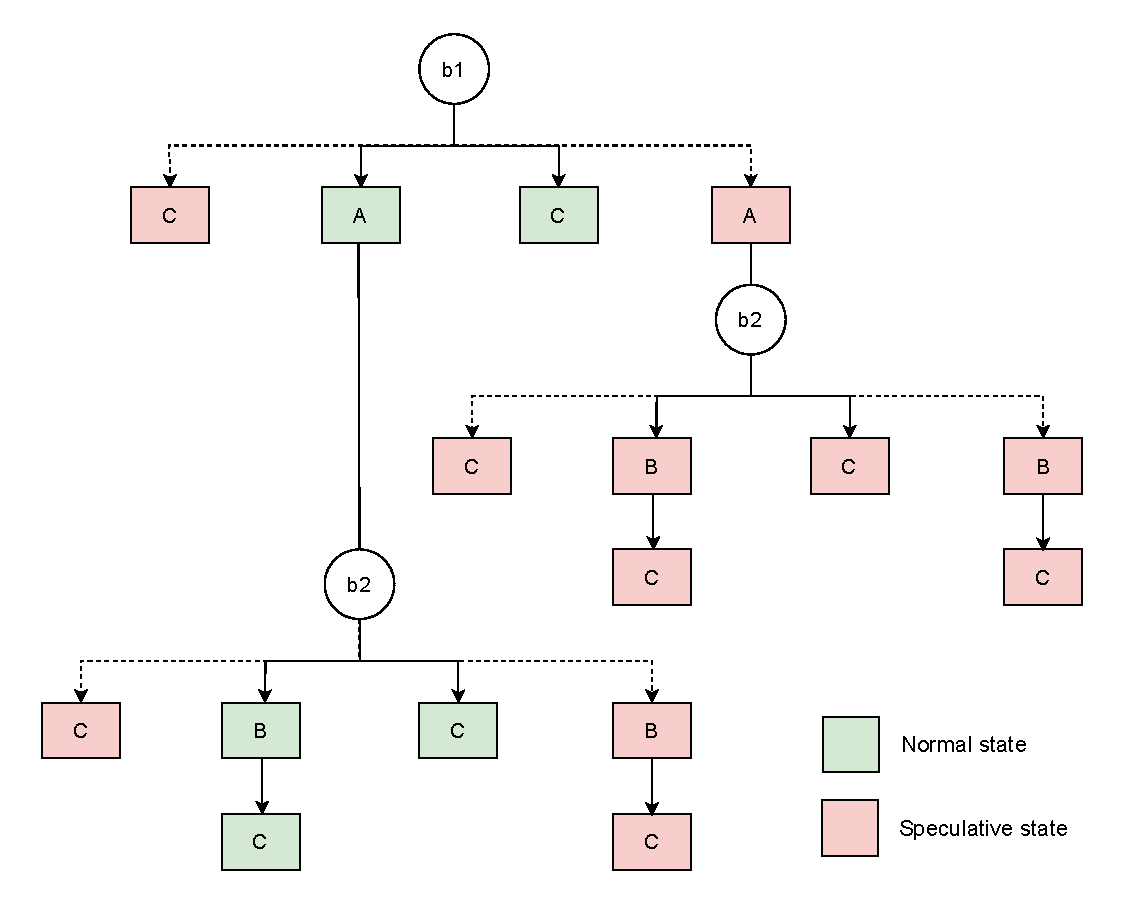
\includegraphics[width=\linewidth]{img/klee_CFG.drawio.pdf}
  \caption{投機的なパスを含んだ制御フローグラフ}
  \label{fig:klee_cfg}
\end{figure}


(1)の場合、KLEESpectreは現在の状態のパス制約に\var{x < SIZE}を追加し、基本ブロック\var{A}に移動し、実行を続ける。
(2)の場合も同様に、現在の状態のパス制約に\var{x >= SIZE}を追加し、基本ブロック\var{C}に移動し、実行を続ける。
(3)の場合、KLEESpectreは現在の状態のパス制約に\var{x < SIZE}を追加するが、分岐予測ミスにより、基本ブロック\var{C}に移動し、実行を続ける。
(4)の場合も同様に、現在の状態のパス制約に\var{x >= SIZE}を追加するが、分岐予測ミスにより、基本ブロック\var{A}に移動し、実行を続ける。このようにKLEESpectreは分岐予測ミスによる投機的なパスも考慮して記号実行を行うようにKLEEを拡張している。図\ref{fig:klee_cfg}において、投機的なパスも含めた図\ref{klee_code}の制御フローグラフを示す。\par
図\ref{fig:klee_cfg}では、実線が直前の分岐命令が正しく分岐予測された場合のパスを、点線が直前の分岐命令が誤って分岐予測された場合の投機的なパスを表している。緑色の基本ブロックは通常の実行パスにおける基本ブロックを、赤色の基本ブロックは投機的なパスにおける基本ブロックを表している。KLEESpectreは全ての分岐命令が攻撃者によって訓練されていると仮定し、投機実行のシミュレートを行う。このシミュレーションにおいて、投機的な状態が以下のいずれかの条件を満たした場合、CPUにおける投機実行の終了動作を再現するためにその状態を破棄する。\par
\begin{itemize}
  \item 投機的なパス上で実行した命令数が投機ウィンドウの制限に達した場合
  \item 直列化命令に遭遇した場合
  \item 例外が発生した場合
\end{itemize}

また、本研究のテーマと関連する重要な点として、KLEESpectreでは分岐予測ミスをネストしてシミュレートする場合がある。図\ref{klee_code}では、分岐\var{b1}の分岐予測ミスによる投機実行中に分岐\var{b2}に遭遇した場合、KLEESpectreは重ねて分岐\var{b2}の分岐予測ミスをシミュレートする。このように、KLEESpectreでは、ある分岐命令の分岐予測ミスから開始された投機実行中に、別の分岐命令に遭遇した場合、重ねて分岐予測ミスをシミュレートする。実際のCPUにおいても、このようなネストされた分岐予測ミスによる投機実行は可能であり\cite{mambretti2019speculator}、KLEESpectreは正しくCPUの投機実行をシミュレートしていると言える。\par
次に、KLEESpectreがどのようにSpectre Gadgetを検出するかについて説明する。
まず、投機的に実行されたパスにおけるメモリアクセスを監視し、それらが秘密情報を参照している場合、その命令をRS(Read Secret)として記録する。KLEESpectreでは、投機的パスにおいて攻撃者が操作可能な値(つまり記号変数)をアドレスとして使用した境界外のメモリアクセスは、すべて秘密情報を参照していると仮定し、保守的な解析を行っている。境界外のメモリアクセスはKLEEに組み込まれているチェック機構を利用して、識別している。次に、秘密情報に依存する値を用いてメモリアクセスが行われた場合、その命令をLS(Leak Secret)として記録する。LSが検出されると、直前に分岐予測ミスが発生した分岐命令と、RSおよびLSに該当する命令のセットをまとめて、Spectre Gadgetとして記録する。\par

KLEESpectreは記号実行を活用することで、単純な静的解析手法に比べて正確であり、動的解析手法に比べてプログラムの網羅的な解析が可能である。これにより、より高い精度でSpectre Gadgetを検出できる。しかし、大規模なコードや探索すべきパスが多い複雑なプログラムに対しては、スケールしないという問題がある。\par

\subsubsection{SpecFuzz}
\label{sec:specfuzz}

\begin{figure}[tb]
  \centering
  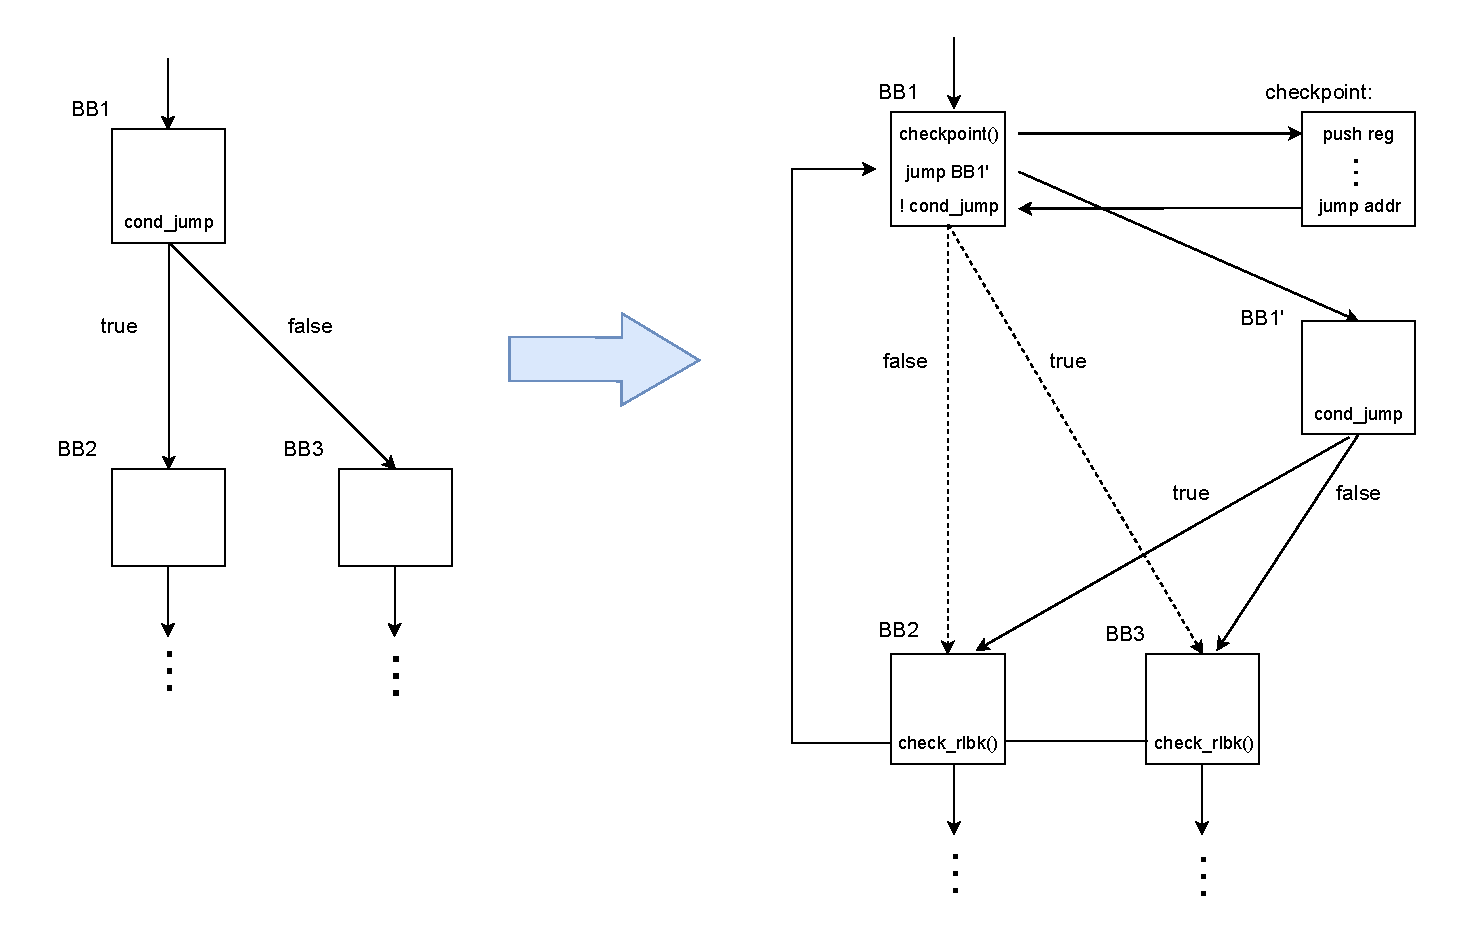
\includegraphics[width=\linewidth]{img/specfuzz_instrument.drawio.pdf}
  \caption{SpecFuzzによる計装前と計装後の制御フローグラフの概略}
  \label{fig:specfuzz_instrument}
\end{figure}


SpecFuzz\cite{oleksenko2020specfuzz}は、ファジングを利用してプログラム内のSpectre Gadgetを検出するためのツールである。ファジングとは、プログラムにランダムに生成された入力を与えることで、バグや脆弱性を検出する動的解析手法である。ファザーは、文法に基づいてゼロからランダムな入力を生成するか、既存のシードを変更して新たなテストケースを作成する。これらの生成されたテストケースをプログラムに与え、その挙動を監視することで、バグや脆弱性を特定する。また、ファジングの重要なパラメーターの1つにカバレッジがある。これは、ファジング中にプログラムがどの程度広範囲にテストされたかを示している。一般的には、ファジング中に少なくとも 1 回実行された制御フローグラフのエッジ数とプログラム内のエッジの合計数の比率として定義される。当然カバレッジが低いと検出対象の見逃しが発生するため、カバレッジを向上させることが多くのファザーにとって重要である。\par
まず、SpecFuzzがどのように分岐予測による投機実行をシミュレートしているかを説明する。SpecFuzzは、テスト対象のプログラムに対してx86アーキテクチャ用のLLVMコンパイラバックエンドパスを利用し、投機実行のシミュレーションに必要なコードを計装する。図\ref{fig:specfuzz_instrument}に計装前のプログラムの制御フローグラフとSpecFuzzによる計装後の制御フローグラフの概略図を示す。点線が分岐予測ミスによるパス、実線が通常の実行によるパスを表している。
また、KLEESpectreと同様に、全ての分岐命令が攻撃者によってトレーニングされていると仮定し、投機実行をシミュレートする。\par
SpecFuzzでは、まず全ての条件分岐命令の直前にチェックポイントを配置する関数(\var{checkpoint})の呼び出しを挿入する。この関数は、投機実行のシミュレーションの開始地点を示し、シミュレーション終了後に通常の実行パスへ戻るため、現在のCPU状態を保持する役割を持つ。具体的には、以下の情報をスナップショットとして取得し、メモリに保存する。\par

\begin{itemize}
  \item レジスタ値(GPR、フラグ、SIMD、浮動小数点レジスタなど)
  \item ロールバック先のアドレス
  \item メタデータ (スタックポインタ、シミュレーション中に実行した命令数など)
\end{itemize}

次に、全ての分岐命令(\var{cond\_jump})を、その分岐条件を反転させた命令(\var{!cond\_jump})に置き換える。この操作により、分岐命令に遭遇するたびに通常の実行パスとは逆方向に処理が進み、投機実行のシミュレーションが開始する。さらに、メモリを変更する全ての命令(mov, push, callなど)の直前には、変更対象のアドレスとその直前の値を記録するコードを挿入する。これにより、投機実行のシミュレーション中に行われた全てのメモリの変更がログに記録され、ロールバック時にシミュレーション開始時点の状態に戻すことが可能になる。\par
投機実行のシミュレーションは、Machine IR(MIR)レベルで実行された命令数が投機ウィンドウによる上限に達するか、直列化命令に遭遇した場合に終了する。各基本ブロックの最後では、シミュレーション中に実行された命令数が投機ウィンドウに達しているかをチェックする関数(\var{check\_rlbk})の呼び出しを挿入する。上限に達していない場合、シミュレーションは継続される。一方で、上限に達していた場合、シミュレーションを終了し、直前のチェックポイント地点にシャンプし、スナップショットに基づいてレジスタやメモリの状態を復元した後、正しい実行パスを再開する。\par
次に、SpecFuzzがどのようにSpectre Gadgetを検出するかについて説明する。SpecFuzzは、投機実行のシミュレーション中に境界外アクセスが検出された場合、その直前に分岐予測ミスが発生した分岐命令と、境界外アクセスが行われた命令を合わせてSpectre Gadgetとして報告する。境界外アクセスの検出には、AddressSanitizer(ASan)\cite{serebryany2012addresssanitizer}が使用される。
この手法は境界外アクセスが攻撃者の操作している値に依存しているかや、境界外アクセスで読み取った値がキャッシュへ転送されるか(LSが存在するか)といったことは考慮されておらず、単純な検出手法である。そのため、実際には攻撃に利用できないGadgetも多数検出される可能性がある\cite{qi2021spectaint}。また、本研究の提案手法とも関連する点として、SpecFuzzはネストされた分岐予測ミスによって悪用可能なGadgetが少ないという観測に基づき、ネストされた分岐予測ミスのシミュレーションを抑制している。そのため、複数回の分岐予測ミスを必要とするGadgetが多数存在した場合、false negativeが増加する。しかし、これらの手法によって、他のファジングベースのSpectre Gadgetの検出手法\cite{qi2021spectaint,johannesmeyer2022kasper}と比較して、より高いファジングスループットを実現している。\par

SpecFuzzはファジングを活用することで、記号実行を用いた手法と比較して大規模なプログラムに対してもスケールする。しかし、ファジング固有の問題であるカバレッジ不足により、一部のSpectre Gadgetを見逃す可能性がある。また、検出機構が単純化されているため、実際には攻撃に利用できないGadgetが誤って検出される可能性もある。
